\section[VHSIC Hardware Description Language (VHDL)]{
  VHSIC Hardware Description Language (VHDL)
  % \texttt{VHDL}: Very high-speed integrated circuits program
  % Hardware Description Language
}

\subsection{Basic syntax and identifiers}
In VHDL an identifier is a case insensitive string composed of
\texttt{A-Z a-z 0-9 \_} that
\begin{itemize}
  \item is not a keyword,
  \item does not start with a number or \texttt{\_},
  \item does not have two or more \texttt{\_} in a row.
\end{itemize}
Expressions are terminated by a semicolon \texttt{;}.
Two dashes in a row cause the rest of the line to be interpreted as a comment.
\begin{lstlisting}[language=vhdl]
expression; -- comment
\end{lstlisting}

\subsection{Structure and Libraries}
The VHDL code is organized into \emph{libraries} declared with the
\vhdl{library} keyword. The library of your code is called \texttt{work},
standard features (\texttt{bit}, \texttt{integer}, \ldots) are found in
\texttt{std}, and IEEE standard parts are in \texttt{ieee}. \texttt{work} and
\texttt{std} are always implicit and must not be declared.
\begin{lstlisting}[language=vhdl]
library `\reqph{library name}`;
\end{lstlisting}
Once declared a library is composed of \emph{packages}, which can contain
elements (constants, entities, \ldots). To access the elements the syntax is 
\begin{lstlisting}[language=vhdl]
`\reqph{library}`.`\reqph{package}`.`\reqph{element}`;
\end{lstlisting}
To avoid having to write a long name every time it is possible to import names
using
\begin{lstlisting}[language=vhdl]
use `\reqph{library}`.`\reqph{element or {\tt all}}`;
use `\reqph{library}`.`\reqph{package}`.`\reqph{element or {\tt all}}`;
\end{lstlisting}

\subsection{Entities and Architectures}
In VHDL the concept of \emph{entity} describes a black box of which only
inputs and outputs are known. The internals of an entity are described through
an \emph{architecture}. There can be multiple architectures for a single entity.

\begin{center}
  \ttfamily
  \begin{tikzpicture}[
      node distance = 1mm,
      pin/.style = {
        draw = black, fill = white, circle, thick,
        inner sep = 0pt, minimum size = 2mm,
      },
    ]
    \node[
      rectangle, draw = black, thick, fill = gray!20!white,
      minimum width = 4.5cm, minimum height = 4cm,
    ] (entity) {};

    \node[anchor = south west] at (entity.north west) {Entity};

    \foreach \x in {1,2,3}{
      \node[
        rectangle, draw = black, thick, fill = white,
        minimum width = 3.5cm, minimum height = .75cm,
      ] (arch\x) at ($(entity.north) + (0, -1 * \x)$) {Architecture \x};
    }

    \foreach \x in {1,...,4}{
      \draw[thick]
        ($(entity.north west) - (0, .75 * \x)$) 
        node[pin] {} to ++(-.75, 0) node (pinl\x) {};

      \draw[thick]
        ($(entity.north east) - (0, .75 * \x)$)
        node[pin] {} to ++(.5, 0) node (pinr\x) {} ;
    }

    \node[right] at (pinr1) {Pin};
  \end{tikzpicture}
\end{center}

Entities are declared with \vhdl{port()} that may contain a list of pins. Pins
have a mode that can be \vhdl{in} input (only LHS\footnote{Left hand side}),
\vhdl{out} output (only RHS\footnote{Right hand side}), \vhdl{inout}
bidirectional or \vhdl{buffer} that can stay both on LHS and RHS. The usage of
the latter is discourareged in favour of an internal signal.
\begin{lstlisting}[language=vhdl]
entity `\reqph{name}` is
  port(
    `\reqph{pin}` : `\reqph{mode} \reqph{type}`;
    `\optionalph{more pins}`;
    `\reqph{pin}` : `\reqph{mode} \reqph{type}`
  );
end entity `\optionalph{name}`;
\end{lstlisting}

Architectures are normally named after the design model, examples are
\texttt{behavioral}, \texttt{structural}.
\begin{lstlisting}[language=vhdl]
architecture `\reqph{name}` of `\reqph{entity}` is
  -- declare used variables, signals and component types
begin
  -- concurrent area
end architecture `\optionalph{name}`;
\end{lstlisting}

\subsection{Electric types}
VHDL provides some types such as
\begin{itemize}
  \item \vhdl{boolean} true or false,
  \item \vhdl{bit} 0 or 1,
  \item \vhdl{bit_vector} one dimensional array of bits,
  \item \vhdl{integer} 32-bit binary representation of a value.
\end{itemize}
From external libraries other types are available:
\begin{itemize}
  \item \vhdl{std_logic} advanced logic with 9 states,
  \item \vhdl{std_ulogic} same as the previous but \emph{unresolved}.
\end{itemize}
The above are from the \vhdl{ieee.std_logic_1164} library, and can take the
values described in the following table.
\begin{center}
  \begin{tabularx}{\linewidth}{>{\ttfamily}c l X}
    \toprule
    Value & Meaning & Usage \\
    \midrule
    U & Uninitialized  & In the simulator \\
    X & Undefined      & Simulator sees a bus conflict \\
    0 & Force to 0     & Low state of outputs \\
    1 & Force to 1     & High state of outputs \\
    Z & High Impedance & Three state ports \\
    W & Weak Unknown   & Simulator sees weak a bus conflict \\
    L & Weak Low       & Open source outputs with pull-down resistor \\
    H & Weak High      & Open drain output with pull-up resistor \\
    - & Don't care     & Allow minimization \\
    \bottomrule
  \end{tabularx}
\end{center}
For the \emph{resolved} types, i.e. \vhdl{std_logic} types, when a signal is
multiply driven the conflict is resolved according to the table below.
Unresolved types will give a synthesization error.
\begin{center}
  \ttfamily
  \begin{tabular}{c|ccccccccc}
    \toprule
      & U & X & 0 & 1 & Z & W & L & H & - \\
    \midrule
    U & U & U & U & U & U & U & U & U & U \\
    X & U & X & X & X & X & X & X & X & X \\
    0 & U & X & 0 & X & 0 & 0 & 0 & 0 & X \\
    1 & U & X & X & 1 & 1 & 1 & 1 & 1 & X \\
    Z & U & X & 0 & 1 & Z & W & L & H & X \\
    W & U & X & 0 & 1 & W & W & W & W & X \\
    L & U & X & 0 & 1 & L & W & L & W & X \\
    H & U & X & 0 & 1 & H & W & W & H & X \\
    - & U & X & X & X & X & X & X & X & X \\
    \bottomrule
  \end{tabular}
\end{center}
A good example is a tri-state bus: 
\begin{lstlisting}[language=vhdl]
architecture tristate of buscontrol is
begin
  bus_read: inp <= bus_io;

  bus_write: process(enable, oup)
  begin
    bus_io <= (others => 'Z');
    if enable = '1' then
      bus_io <= oup;
    end if;
  end process;
end architecture tristateout;
\end{lstlisting}

\subsection{Declarations} \label{sec:declarations}
Before a \vhdl{begin} -- \vhdl{end} block, there is usually a list of declarations.
A self evident examples are \emph{constants}.
\begin{lstlisting}[language=vhdl]
constant `\reqph{name}` : `\reqph{type}` := `\reqph{value}`;
\end{lstlisting}

Next, \emph{signals} and \emph{variables}. Signals is are wires, they can only be
connected and do not have an initial state. Variables can be assigned like in
software, but can cause the synthesization of an unwanted D-Latch.

\begin{lstlisting}[language=vhdl]
signal `\reqph{name}`, `\optionalph{name, \ldots}` : `\reqph{type}`;

variable `\reqph{name}`, `\optionalph{name}`, `\optionalph{\ldots}` : `\reqph{type}`;
variable `\reqph{name}` : `\reqph{type}` := `\reqph{expression}`;
\end{lstlisting}

For the hierarchical designs, when external entities are used, they must be
declared as components. The \vhdl{port()} expression must match the entity
declaration.
\begin{lstlisting}[language=vhdl]
component `\reqph{entity name}` is
  port(
    `\optionalph{list of pins}`
  );
end component;
\end{lstlisting}
For entities with multiple architectures, it is possible to choose which
architecture is used with the following expression.
\begin{lstlisting}[language=vhdl]
for `\reqph{label or {\tt all}}`: use entity `\reqph{library}`.`\reqph{entity}`(`\reqph{architecture}`);
\end{lstlisting}

\subsection{Concurrent Area}
\begin{center}
  \ttfamily
  \begin{tikzpicture}[
      node distance = 1mm,
      pin/.style = {
        draw = black, fill = white, circle, thick,
        inner sep = 0pt, minimum size = 2mm,
      },
      component/.style = {
        draw = black, thick, fill = white, rectangle,
        minimum width = 18mm, minimum height = 12mm,
        align = center,
      },
    ]

    \node[
      draw = black, rectangle, fill = gray!20!white, thick,
      minimum width = .75\linewidth, minimum height = 4cm,
    ] (arch) {};

    \node[anchor = south west] at (arch.north west) {Architecture};

    \node[pin] (clk) at ($(arch.north west) - (0,1)$) {};
    \node[pin] (a) at ($(clk) - (0,1)$) {};
    \node[pin] (b) at ($(a) - (0,1)$) {};
    \node[pin] (y) at ($(arch.north east) - (0,1)$) {};

    \node[left = of clk] {clk};
    \node[left = of a] {a};
    \node[left = of b] {b};
    \node[right = of y] {y};

    \node[component] (c1) at ($(clk) + (2,-.2)$) {Process};
    \node[component] (c2) at ($(c1) + (.2,-1.8)$) {Component\\ (entity)};
    \node[
      component, minimum width = 0mm, minimum height = 0mm,
    ] (c3) at ($(c1) + (2.6,-.2)$) {Logic\\ Gate};

    \draw[thick]
      (clk)     to[out = 0, in = 180] ($(c1.west) + (0,.2)$)
      (a)       to[out = 0, in = 180] ($(c1.west) - (0,.2)$)
      (b)       to[out = 0, in = 180] (c2.west)

      (c1.east) to[out = 0, in = 180] ($(c3.west) + (0,.2)$)
      (c2.east) to[out = 0, in = 180] ($(c3.west) - (0,.2)$)
      (c3.east) to[out = 0, in = 180] (y)
      ;

  \end{tikzpicture}
\end{center}

In the architecture between \vhdl{begin} and \vhdl{end}, the expressions
are \emph{not} read sequentially, everything happens at the same time.
Statements inside the concurrent area optionally have a label.
\begin{lstlisting}[language=vhdl]
`\optionalph{label}`: `\reqph{concurrent statement}`;
\end{lstlisting}
In the concurrent area signals, components and processes can be used to create
a logic.

\subsubsection{Signal assignment and simple gates}
Signals are assigned using \vhdl{<=}.
\begin{lstlisting}[language=vhdl]
`\optionalph{label}`: `\reqph{signal}` <= `\reqph{expression}`;
\end{lstlisting}
Simple logic functions such as \vhdl{not}, \vhdl{and}, \vhdl{or}, \vhdl{xor},
etc. can be used.
\begin{lstlisting}[language=vhdl]
 y <= (a and s) or (b and not(s));
\end{lstlisting}

\subsubsection{Aggregates}
For vector types it is possible to create a value out of multiple signals.
\begin{lstlisting}[language=vhdl]
`\reqph{vector}` <= (
  `\reqph{index}`  => `\reqph{source or value}`,
  `\reqph{index}`  => `\reqph{source or value}`,
  `\optionalph{\tt others}` => `\reqph{source or value}`
);
\end{lstlisting}
\begin{lstlisting}[language=vhdl]
-- declaration
signal data : bit_vector(6 downto 0);
signal a, b : bit;
\end{lstlisting}
\begin{lstlisting}[language=vhdl]
-- concurrent
data = (1 => a, 0 => b, others => '0')
\end{lstlisting}

\subsubsection{Selective and conditional assignment}
Higher level conditions can be written in two ways. 
\begin{lstlisting}[language=vhdl]
-- using when
`\optionalph{label}:` y <= `\reqph{source}` when `\reqph{condition}` else
     `\reqph{source}` when `\reqph{condition}` else
     `\reqph{source}` when `\reqph{condition}`;
\end{lstlisting}
\begin{lstlisting}[language=vhdl]
-- using with
`\optionalph{label}`: with `\reqph{signal}` select `\reqph{dest}` <= 
  `\reqph{source}` when `\reqph{value}`,
  `\reqph{source}` when `\reqph{value}`,
  `\reqph{source}` when others;
\end{lstlisting}

\subsubsection{Components}
External components that have been previously declared can be used with the
\vhdl{port map(}\reqph{assignments}\texttt{)} syntax. For example:
\begin{lstlisting}[language=vhdl]
-- declaration
component flipflop is
  port(
    clk, set, rst : in  std_ulogic,
    Q, Qn         : out std_ulogic 
  );
end component flipflop;

signal clk_int, a, b : in  std_ulogic;
signal y, z          : out std_ulogic;
\end{lstlisting}
\begin{lstlisting}[language=vhdl]
-- concurrent
u1: component flipflop
  port map(
    clk => clk_int,
    set => a,
    rst => b,
    Q   => y,
    Qn  => z
  );

\end{lstlisting}

\subsubsection{Processes}
For more sophisticated logic VHDL offers a way of writing sequential statements
called \emph{process}.
\begin{lstlisting}[language=vhdl]
`\optionalph{label}:` process (`\optionalph{sensitivity list}`)
-- declarations
begin
  -- sequential statements
end process;
\end{lstlisting}
Processes have a \emph{sensitivity list} that can be empty.  When a signal in
the sensitivity list changes state, the process is executed.  With an empty
sensitivity list, the process runs continuously.  In the declaration,
everything from \S\ref{sec:declarations} applies. For the sequential
statements, the following applies:
\begin{itemize}
  \item Neither selective (\vhdl{with}) nor conditional (\vhdl{when}) should be used.
    They are replaced with new sequential constructs (\vhdl{if} and \vhdl{case}).
  \item Signal assignments (with \vhdl{<=}) change their value
    \emph{only at the end of the process}.
  \item Variables on the other hand change as soon as they are assigned (with \vhdl{:=}).
\end{itemize}
And for good practice:
\begin{itemize}
  \item Before any \vhdl{if} or \vhdl{case} default values should be assigned.
  \item Any signal on the RHS should be in the sensitivity list.
  \item Processes with empty sensitivity lists should only be used for simulations.
\end{itemize}

The sequential replacements for \vhdl{with} and \vhdl{when} are in the listings below.
\begin{lstlisting}[language=vhdl]
if `\reqph{condition}` then
  -- sequential statements 
elsif `\reqph{condition}` then
  -- sequential statements 
else
  -- sequential statements 
end if;
\end{lstlisting}
\begin{lstlisting}[language=vhdl]
case `\reqph{expression}` is
  when `\reqph{choice}` =>
    -- sequential statements
  when `\reqph{choice}` =>
    -- sequential statements
  when others =>
    -- sequential statements
end case;
\end{lstlisting}

Processes can detect \emph{attributes} of signals. Typically it is used for
clocks. There are also other attributes such as \vhdl{s'stable(t)}.
\begin{lstlisting}[language=vhdl]
process (clk)
begin
  -- rising edge
  if clk'event and clk = '1' then
    ... end if;
  if rising_edge(clk) then
    ... end if;

  -- falling edge
  if clk'event and clk = '0' then
    ... end if;
  if falling_edge(clk) then
    ... end if;
end process;
\end{lstlisting}

\subsection{Custom and arithmetic types}
It is possible to create custom types, usually to create state machines.
\begin{lstlisting}[language=vhdl]
type `\reqph{name}` is (`\reqph{identifier}`, `\reqph{identifier}`, `\ph{\ldots}`);
\end{lstlisting}

\subsection{Pitfalls and RTL model}
Coming from a programming language, a common pitfall is to write something like
\begin{center}
  \begin{minipage}{.4\linewidth}
    \begin{lstlisting}[language=vhdl]
-- wrong!!!
y <= y xor a;
    \end{lstlisting}
  \end{minipage}
  \begin{minipage}{.4\linewidth}
    \centering
    \ttfamily
    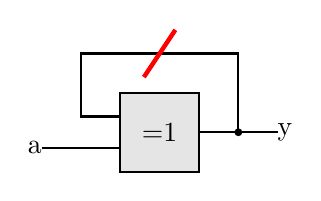
\begin{tikzpicture}[
        outer sep = 0mm, inner sep = 0mm,
        comp/.style = {
          rectangle, draw = black, thick, fill = gray!20!white,
          minimum height = 1cm, minimum width = 1cm,
        }
      ]

      \node[comp] (G) {=1};
      \draw[thick] (G.west) ++(0,-.2) to ++(-1,0) node[left] {a};
      \draw[thick] (G.west) ++(0,.2) 
        to ++(-.5,0)
        to ++(0,.8)
        to ++(2,0)
        to ++(0,-1) node[minimum size = 1mm, fill = black, circle] (n) {}
        to ++(-.5,0);

      \draw[thick] (n) to ++(.5,0) node[right] {y};

      \draw[ultra thick, red] (G.north) ++(-.2,.2) to ++(.4,.6);
      % \draw[ultra thick, red] (G.north) ++(.2,.2) to ++(-.4,.6);
    \end{tikzpicture}
  \end{minipage}
\end{center}
but this will be synthesised into an oscillating circuit, that must be avoided
at all costs. The correct way is to have a memory for the next state, with a
logic separated into combinatorial and sequential parts.
\begin{lstlisting}[language=vhdl]
-- combinatorial
y_next <= y xor a;
-- sequential
process (clk)
begin
  if rising_edge(clk) then
    y <= y_next;
  end if;
end process;
\end{lstlisting}
This method is known as \emph{register transfer level} design.

\subsection{Generic Parameters}
Sometimes a group of components have a very similar structure, so instead of
rewriting multiple similar interfaces it is desirable to have \emph{parameters}
and a \emph{generic} entity, for example in the case of a binary counter's
range. To solve the problem using signals with conditional statements would
generate unnecessary hardware, while constants cannot change the entity's port.
Thus there is a syntax:
\begin{lstlisting}[language=vhdl]
generic(
  `\reqph{param name}` : `\reqph{type}` := `\reqph{initial value}`;
  `\optionalph{more parameters}`;
  `\reqph{param name}` : `\reqph{type}` := `\reqph{initial value}`
);
\end{lstlisting}
that has affects at \emph{synthesization time}.

\subsubsection{Generic entity and declaration}
Entities are parametrized as follows.
\begin{lstlisting}[language=vhdl]
entity `\reqph{name}` is
  generic(`\reqph{parameters}`);
  port(`\reqph{pins}`);
end entity `\reqph{name}`;
\end{lstlisting}
For example:
\begin{lstlisting}[language=vhdl]
entity counter is
  generic(CNT_MAX : natural := 127);
  port(
    clk, rst, ena : in std_logic;
    -- adjust to a power of 2
    count : out std_logic_vector(
      (natural(ceil(
        log2(real(CNT_MAX +1)))) -1)
        downto 0);
end entity;
\end{lstlisting}
And in the architecture it is possible to access generic values in a similary
way. Another example is a clock divider.
\begin{lstlisting}[language=vhdl]
entity clockdivider is
  generic(DIV_FACTOR : natural := 128);
  port(...);
end entity;

architecture RTL of clockdivider is
  signal cnt, cnt_next : natural range 0 to (DIV_FACTOR -1);
  ...
\end{lstlisting}

\subsubsection{Generic mapping (Concurrent Area)}
To map a generic entity into a structural design the syntax is extended
accordingly with \vhdl{generic map()}.
\begin{lstlisting}[language=vhdl]
-- definition
component `\reqph{generic entity}` is
  generic(`\reqph{parameters}`);
  port(`\reqph{pins}`);
end component;
\end{lstlisting}
\begin{lstlisting}[language=vhdl]
`\optionalph{label}`: component `\reqph{generic component}`
  generic map(
    `\reqph{parameter}` => `\reqph{constant or parameter}`,
    ...
  );
  port map(
    `\reqph{pin}` => `\reqph{signal or pin}`, 
    ...
  );

\end{lstlisting}

% vim:ts=2 sw=2 et:
